\chapter{Quantum Chromodynamics}\label{chap:qcd}
Quantum chromodynamics, the theory of strong interactions, was developed on the basis of scattering experiments that showed the existence of an internal $SU(3)$-symmetry and related (color) charges \cite{NPgaugeLecture} and has been subject to intense research over the last decades. \\
This chapter serves as an introduction to the theoretical formalism behind QCD, most of the treated subjects are textbook knowledge on the level of an advanced QFT course, cf. \cite{NPgaugeLecture, QFTNotesFloerchingerWetterich, QFTNotesPawlowskiJaeckel, PawlowskiPlehnQCD} for lecture notes  or \cite{Muta2010, PeskinSchroeder1995, ItzyksonZuber1980, Thomson2013, Georgi1999} for very detailed textbooks.\\
 Note, that we do not aim to provide a complete introduction to the subject but rather focus on the non-perturbative aspects of the theory to make the reader familiar with the concepts required for a general understanding of the conducted calculations.\\
We will briefly recap the most important steps in the quantization of general non-Abelian gauge theories, introduce the superfield formalism to condense our notation and derive the actions for pure Yang-Mills theory and QCD. We conclude our discussion by presenting the Dyson-Schwinger equations for the gluon, ghost and quark propagators, respectively,  as they are the central functional relations in the context of our work.\\
Concerning notational conventions we again closely follow \cite{NPgaugeLecture} and \cite{Cyrol2017}.


\section{Non-Abelian Gauge Theories and Yang-Mills Theory}\label{sec:yang_mills}
Compared to Abelian theories such as Quantum Electrodynamics (QED) with gauge group $U(1)$ related to the electric charge, the underlaying gauge theory of QCD, $SU(3)$ Yang-Mills theory, is self-interacting and hence already non-trivial on the classical level. The quantization of non-Abelian gauge theories has to be treated very carefully. In the subsequent section we will go through this process and fix our notation.                                                                                                                                                                                                                                                                                                                                                                                                                                                                                                            
\subsection{General Concepts and the Yang-Mills Action}
In general, Lagrangians of physical quantum field theories are constructed such that they are invariant under (gauge) transformations of the respective gauge group. This general requirement and the assumption of minimal coupling leads to the promotion of partial derivatives to covariant derivatives in the following way:
\begin{equation}
\partial_{\mu} \rightarrow D_{\mu}(A) = \partial_{\mu} - igA_{\mu},	\label{eqn:covariant_derivative}
\end{equation}
with the strong coupling constant $g=\sqrt{4\pi\alpha}$ and the matrix-valued gauge field
\begin{equation}
A_{\mu}=A_{\mu}^{a} T^{a} \in \mathfrak{su}(N_c), 
\end{equation}
with the $N_c^2-1$ generators $T^{a}$ of the associated Lie algebra $\mathfrak{su}(N_c)$. For $SU(3)$, the relevant gauge group for QCD,  the $T^{a}$ are the Gell-Mann matrices $\lambda^{a}, \ a\in\left\{1,\dots 8\right\}$, explicitly

\begin{equation}
	\begin{aligned}
\lambda_1 &= \begin{pmatrix} \phantom{-}0 & \phantom{-}1 & \phantom{-}0\phantom{-} \\ \phantom{-}1 & \phantom{-}0 & \phantom{-}0\phantom{-} \\ \phantom{-}0 & \phantom{-}0 & \phantom{-}0\phantom{-} \end{pmatrix},\
\lambda_2 = \begin{pmatrix} \phantom{-}0 & -i & \phantom{-}0\phantom{-} \\ \phantom{-}i & \phantom{-}0 & \phantom{-}0\phantom{-} \\ \phantom{-}0 & \phantom{-}0 & \phantom{-}0\phantom{-} \end{pmatrix} ,\
\lambda_3 = \begin{pmatrix} \phantom{-}1 & \phantom{-}0 & \phantom{-}0\phantom{-} \\ \phantom{-}0 & -1 & \phantom{-}0\phantom{-} \\ \phantom{-}0 & \phantom{-}0 & \phantom{-}0\phantom{-} \end{pmatrix}, \\[0.5em]
\lambda_4 &= \begin{pmatrix} \phantom{-}0 & \phantom{-}0 & \phantom{-}1\phantom{-} \\ \phantom{-}0 & \phantom{-}0 & \phantom{-}0\phantom{-} \\ \phantom{-}1 & \phantom{-}0 & \phantom{-}0\phantom{-} \end{pmatrix},\ 
\lambda_5 = \begin{pmatrix} \phantom{-}0 & \phantom{-}0 & -i\phantom{-} \\ \phantom{-}0 & \phantom{-}0 & \phantom{-}0\phantom{-} \\ \phantom{-}i & \phantom{-}0 & \phantom{-}0\phantom{-} \end{pmatrix},\
\lambda_6 = \begin{pmatrix} \phantom{-}0 & \phantom{-}0 & \phantom{-}0\phantom{-} \\ \phantom{-}0 & \phantom{-}0 & \phantom{-}1\phantom{-} \\ \phantom{-}0 & \phantom{-}1 & \phantom{-}0\phantom{-} \end{pmatrix}, \\[0.5em]
\lambda_7 &= \begin{pmatrix} \phantom{-}0 & \phantom{-}0 & \phantom{-}0\phantom{-} \\ \phantom{-}0 & \phantom{-}0 & -i\phantom{-} \\ \phantom{-}0 & \phantom{-}i & \phantom{-}0\phantom{-} \end{pmatrix},\
\lambda_8 = \frac{1}{\sqrt{3}} \begin{pmatrix} \phantom{-}1 & \phantom{-}0 & \phantom{-}0\phantom{-} \\ \phantom{-}0 & \phantom{-}1 & \phantom{-}0\phantom{-} \\ \phantom{-}0 & \phantom{-}0 & -2\phantom{-} \end{pmatrix}.
	\end{aligned}\label{eqn:Gell-Mann}
\end{equation}
The fact, that the gauge fields are matrix-valued and therefore do not trivially commute with each other already highlights the main difference to the Abelian case, that the gauge field is self-interacting.
The generators satisfy the commutation relation 
\begin{equation}
\left[T^{a}, T^{b}\right]=i f^{a b c} T^{c},
\end{equation}
uniquely defining the structure constants $f^{abc}$ of the Lie algebra. The respective relation in the adjoint representation of the gauge group reads 
\begin{equation}
	\left(T^c_{\mathrm{adj.}}\right)^{ab} = -if^{abc}.
\end{equation}
The normalization of the generators is chosen such that 
\begin{equation}
\operatorname{Tr}_{f}\left[T^{a}, T^{b}\right]=\frac{1}{2} \delta^{a b}.\label{eqn:normalization}
\end{equation}
Note, that the index $f$ here refers to the trace being evaluated in the fundamental representation of the gauge group. Another important quantity related to the gauge group is its quadratic Casimir operator, often referred to as color factor in QCD computations,
\begin{equation}
	C_f(N_c) = T^{a}T^{a} = \frac{N_c^2-1}{2N_c} \equiv \frac{4}{3} \quad\text{for } SU(3).
\end{equation}

With these definitions at hand, we are now ready to construct the explicit gauge transformations and classify the transformation behavior of the gauge and spinor fields $q(x)$\footnote{We did not yet introduce the spinor fields $\psi(x)$ representing the quarks, they will be included after discussing the entire quantization process of the pure gauge sector. Nevertheless, their transformation behavior will already be presented at this point.}, the fundamental degrees of freedom in our theory. Explicitly, local gauge transformations can be written as
\begin{equation}
U(x)=\exp\left[-i g \theta^{a}(x) T^{a}\right] \in S U(N_{c}), \label{eqn:local_gauge_trafo}
\end{equation}
with a real, spacetime-dependent parameter $\theta(x) \in \mathfrak{su}(N_c)$. With the definition in  \eqref{eqn:local_gauge_trafo}, the gauge fields transform in the adjoint and the spinor fields in the fundamental representation according to
\begin{equation}
\begin{aligned}
A_{\mu} \rightarrow A_{\mu}^{\prime} &=U A_{\mu} U^{\dagger} -\frac{i}{g}\left(\partial_{\mu}U\right)U^{\dagger},\\
\psi \rightarrow \psi^{\prime} &=U \psi,\\
\bar{\psi} \rightarrow \bar{\psi}^{\prime} &=\bar{\psi}\ U^{\dagger} 
\end{aligned}
\end{equation}
\begin{figure}[t]
\centering
\begin{align*}
S_{\mathrm{YM}}[A] =
\big(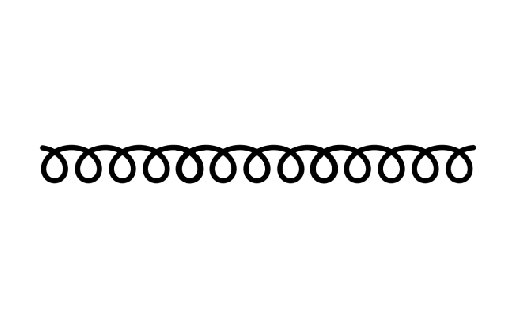
\includegraphics[scale=0.3, valign=c]{figs/diagrams/qcd_action/gluon_propagator}\big)^{-1} +
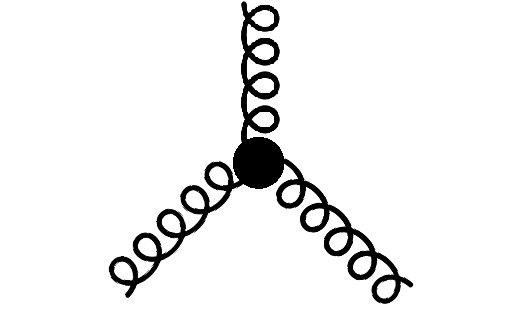
\includegraphics[scale=0.3, valign=c]{figs/diagrams/qcd_action/3gluon_vertex} +
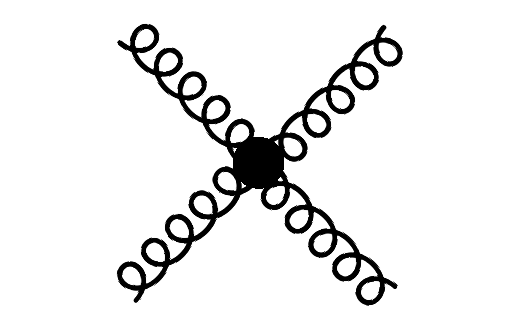
\includegraphics[scale=0.3, valign=c]{figs/diagrams/qcd_action/4gluon_vertex} 
\end{align*}

\caption{Diagrammatical representation of the classical Yang-Mills action featuring the (inverse) gluon propagator and the characteristic cubic and quartic gluon self interactions.}
\label{fig:ym_action}
\end{figure}
\hspace{-0.5em} The gluon field strength tensor $F_{\mu\nu}$ is then constructed as the curvature tensor corresponding to the covariant derivative as usual, i.\,e. 
\begin{equation}
F_{\mu \nu}=\frac{i}{g}\left[D_{\mu}, D_{\nu}\right]=F_{\mu \nu}^{a} T^{a} \quad \text { with } \quad F_{\mu \nu}^{a}=\partial_{\mu} A_{\nu}^{a}-\partial_{\nu} A_{\mu}^{a}+g f^{a b c} A_{\mu}^{b} A_{\nu}^{c},
\end{equation}
and has by construction the desired transformation behavior
\begin{equation}
F_{\mu \nu} \rightarrow F^{\prime}_{\mu \nu}=U F_{\mu \nu}\ U^{\dagger}.
\end{equation}
With this we are finally able to construct the gauge-invariant Yang-Mills action:
\begin{equation}
	S_{\mathrm{YM}}[A] = \frac{1}{2} \int_x \operatorname{Tr}\big[F_{\mu\nu} F_{\mu\nu}\big]\ \overset{(\ref{eqn:normalization})}{=}\  \frac{1}{4} \int_x F_{\mu\nu}^{a} F_{\mu\nu}^{a}.\label{eqn:ym_action}
\end{equation}
Note the factor of $1/2$ coming from the normalization of the generators.
A diagrammatic representation of this action featuring its characteristic properties is presented  in \figref{fig:ym_action}. \\
\noindent Unfortunately we are not finished yet, since the action defined in \eqref{eqn:ym_action} features physically equivalent gauge degrees of freedom, living on the same gauge orbit, i.\,e. all configurations connected via gauge transformations. The next section is denoted to resolve this problem\footnote{This is still not the full solution to the problem, since  we have to be careful with the Gribov ambiguity, i.\,e. that  a gauge fixing submanifold (associated with a specific gauge choice) may not intersect a gauge orbit at all or it may intersect it more than once \cite{Gribov1978}, but we will not focus on this in detail here.} by employing the so-called Faddeev-Popov gauge fixing procedure \cite{FaddeevPopov1967}.
\subsection{Quantization and Gauge Fixing}
As observed before, we have to cope with the fact, that the action (\ref{eqn:ym_action}) features infinitely many redundancies, i.\,e.  physically equivalent field configurations connected via gauge transformations (\ref{eqn:local_gauge_trafo}). 
The general gauge fixing condition can be implemented as
\begin{equation}
\mathcal{F}[A_{\mathrm{gf}} = A^{U(\theta_{\mathrm{gf}})}]=0, \label{eqn:condition}
\end{equation}
with the algebra element $\theta_{\mathrm{gf}}$ being the one that satisfies a certain gauge fixing condition. This corresponds to the explicit choice of one representative per gauge orbit. Concerning this work, we restrict ourselves to the rather general class of linear covariant gauges of the form
\begin{equation}
	\mathcal{F}[A_{\mathrm{gf}}]=l_{\mu}A_{\mu}.
\end{equation}
Here, $l_{\mu}$ can be a differential operator, space-time dependent or a combination thereof \cite{Wink2020}. For a collection of commonly used conventions see below:
\begin{align}
	\mathcal{F}[A_{\mathrm{gf}}]\equiv l_{\mu}A_{\mu},\quad \text{explicitly}\quad \left\{\begin{array}{ll}{\mathcal{F}[A_{\mathrm{gf}}] = \partial_{\mu}A_{\mu},} & {\text{Covariant or Lorenz gauge}} \\ {\mathcal{F}[A_{\mathrm{gf}}] = \partial_iA_i,} & {\text {Coulomb gauge}} \\ {\mathcal{F}[A_{\mathrm{gf}}] = x_{\mu}A_{\mu},} & {\text{Fock-Schwinger gauge}} \\ {\mathcal{F}[A_{\mathrm{gf}}] = n_{\mu}A_{\mu},} & {\text{Axial gauge}} \\ {\mathcal{F}[A_{\mathrm{gf}}]: A_0(x) = A_0^c(\mathbf{x}),} & {\text{Polyakov gauge}}\end{array}\right.
\label{eqn:regulator_limits}
\end{align}
Technically, for a general gauge condition such as in (\ref{eqn:condition}), we can now handle the implementation by splitting the functional integration over the gauge fields into physically inequivalent ($A_{\mathrm{gf}}$) and equivalent, gauge contributions ($\theta$),  
\begin{equation}
\int\mathcal{D} A = \int J\ \mathcal{D}A_{\mathrm{gf}}\ \mathcal{D}\theta, \label{eqn:measure}
\end{equation}
with the Jacobian of the variable transformation $J$ and the so called Haar measure $\mathcal{D}\theta$. Due to the gauge invariance of the action, the integration over the the gauge group factorizes and can be dropped\footnote{Technically, the $\theta$-dependence can be absorbed in $A\rightarrow A^{\theta}$, which directly follows from gauge invariance of the considered quantities. This allows for a cancellation of the respective contributions when computing general observables $\mathcal{O}$. The redundancy is therefore eliminated in the path integral.}. Using the property (\ref{eqn:measure}) and making use of the identity
\begin{equation}
1=\int \mathcal{D} A\ \delta( \mathcal{F})\overset{(\ref{eqn:measure})}{=}\int \mathcal{D} \theta(x)\ \delta\left( \mathcal{F}[A^{\theta}]\right) \operatorname{det}\left(\frac{\delta  \mathcal{F}[A^{\theta}]}{\delta \theta}\right),
\label{eqn:FP_identity}
\end{equation}
where $\delta$ is the functional Dirac delta distribution, we come to the central idea of the Faddeev-Popov trick \cite{FaddeevPopov1967}. The trick is to represent the occurring functional determinant in terms of a Gaussian integral over anti-commuting Grassmann fields, which evaluates for covariant gauges, $\partial_{\mu}A_{\mu}=0$, to 
\begin{equation}
\operatorname{det}\left(\frac{\delta \mathcal{F}^{a}}{\delta \theta^{b}}\right)=\operatorname{det}\left(\frac{1}{g} \partial_{\mu} D_{\mu}^{a b}\right)=\int \mathcal{D} c \mathcal{D} \bar{c}\ \exp \left[\int_{x} \bar{c}^{a} \partial_{\mu} D_{\mu}^{a b} c^{b}\right],
\end{equation}
where we used $\frac{\delta G^{a}}{\delta \theta^{b}}=\frac{\delta G^{a}}{\delta A_{\mu}^{c}} \frac{\delta A_{\mu}^{c}}{\delta \theta^{b}}$ and introduced the covariant derivative in the adjoint representation,
\begin{equation}
D_{\mu}^{a b}=\delta^{a b} \partial_{\mu}-g f^{a b c} A_{\mu}^{c}.
\end{equation}
The fields $c$ and $\bar{c}$ are usually referred to as Faddeev-Popov ghosts and antighosts. They are no physical (= observable) degrees of freedom since they violate the spin statistics theorem. Their sole purpose is to cancel unphysical degrees of freedom and thereby guarantee unitarity \cite{Cyrol2017}. Integrating over the $\delta$-function in (\ref{eqn:FP_identity}) by introducing a Gaussian weighting function of the form 
\begin{equation}
\delta\left[\mathcal{F}[A^{\theta}]\right] \rightarrow \int \mathcal{D}\omega\ \delta\left[\mathcal{F}[A^{\theta}-\omega]\right] \exp \left\{-\frac{1}{2 \xi} \int_{x} \omega^{a} \omega^{a}\right\},
\end{equation}
with arbitrary functions $\omega^{a}(x)$, leads to the explicit appearance of a so called gauge fixing parameter $\xi$ in the theory.
In total, we can now conclude our findings and finally present the expression for the gauge-fixed generating functional of Yang-Mills theory:
\begin{equation}
Z[J]=\int \mathcal{D}A\ \exp \left(S_{\mathrm{YM}}[A]+\int_{x} J_{\mu}^{a} A_{\mu}^{a}\right).
\end{equation}
\paragraph{A Short Introduction to the Superfield Formalism.}

At this point we want to introduce briefly the superfield formalism \cite{QMeS2021, NPgaugeLecture} as a very useful tool to condense our notation in the discussion of the quantization and gauge fixing procedure for general non-Abelian gauge theories. \\
For our concrete example of Yang-Mills theory we collect the field content in a so-called superfield $\Phi = \left(A, c, \bar{c}\right)^T$. The corresponding metric tensor then reads
\begin{equation}
(\gamma)^{a b}=\left(\begin{array}{ccc}
1 & \phantom{-}0 & \phantom{-}0  \\
0 & \phantom{-}0 & \phantom{-}1  \\
0 & -1 & \phantom{-}0  \\
\end{array}\right),
\end{equation}
resulting from  the convention $\Phi_{a}\Phi^{a} = A^2 + 2c\bar{c}$, or in other words the metric $\gamma$ is diagonal in bosonic and symplectic in fermionic subspaces. By convention indices are always raised from the left and lowered from the right, i.\,e.  $\Phi^{a} = \gamma^{ab}\Phi_{b} = \Phi_{b}\gamma^{ab} = \left(A, c, \bar{c}\right)$ which directly implies the following identities:
\begin{align}
	\gamma_{a}^{\phantom{a}b} &= \gamma^{bc}\gamma_{ac} = \delta^{b}_{\phantom{c}a} \\
	\gamma^{a}_{\phantom{a}b} &= \gamma^{ca}\gamma_{bc} = (-1)^{ab}\delta^{a}_{\phantom{c}b},
\end{align}
where 
\begin{equation}
\begin{aligned}
	(-1)^{ab} = \left\{\begin{array}{ll}{-1} & {\text { if } a\ \text{and}\ b \text { fermionic, } } \\ {\phantom{-}1} & {\text { otherwise. }} 
	\end{array}\right.
\end{aligned}
\end{equation}
This condensed notation allows us to write all relevant functionals and equations including sets of multiple fields of different kinds  in a short and concise way.\\
Applying these conventions to our equations leaves us with the following expression for the gauge fixed generating functional for Yang-Mills theory,
\begin{equation}
Z\left[J\right]=\int \dd \Phi\ \exp\left(-S_{\mathrm{YM}}[\Phi]+J_{\Phi}\cdot \Phi\right),
\end{equation}
with the Yang-Mills superfield $\Phi$ as above, and the corresponding supercurrent, 
\begin{equation}
\begin{aligned}
J_{\Phi} &= (J_A, J_c, J_{\bar{c}}).
\end{aligned}
\end{equation}
The gauge-fixed action $S_A$ now features the  gauge fixing and ghost terms, as derived before, 
\begin{equation}
S_{\mathrm{YM}}[\Phi]=\underbrace{\frac{1}{4} \int_{x} F_{\mu \nu}^{a} F_{\mu \nu}^{a}}_{S_{\mathrm{gauge}}}+\underbrace{\frac{1}{2 \xi} \int_{x}\left(\partial_{\mu} A_{\mu}^{a}\right)^{2}}_{S_{\mathrm{gf}}}-\underbrace{\int_{x} \bar{c}^{a} \partial_{\mu} D_{\mu}^{a b} c^{b}}_{S_{\mathrm{gh}}}.
\end{equation}
The explicit choice of the gauge fixing parameter $\xi$ can simplify computations a lot. A common choice for perturbative calculations is $\xi=1$, which is known as \textit{Feynman gauge}. We decided to work in \textit{Landau gauge} corresponding to the choice $\xi=0$, which has to be understood as taking the limit $\xi\rightarrow 0$ after deriving the explicit expressions. For most applications of functional methods Landau gauge is the standard way to go, since it allows for a complete decoupling of the longitudinal and transversal parts  of the respective equations. This will be made clear in the subsequent discussion of our calculations in \chapref{chap:results}.
 

\section{From Yang-Mills to QCD}\label{sec:ym_to_qcd}
Up to now, we only focused on the pure gauge part of the theory. To arrive at the final expression for the full QCD action, we need to introduce quarks. The corresponding action for free quarks is given by the usual Dirac action for fermions, the minimal coupling between the quarks and gluons is again realized by promoting the partial derivatives to covariant ones, cf. (\ref{eqn:covariant_derivative}). This yields
\begin{equation}
S_{\mathrm{Dirac}}[A,\bar{\psi},\psi]=\int_x \bar{\psi}(i\slashed{D} + m_{\psi}) \psi,
\end{equation}
with the spin-$\frac{1}{2}$ spinor fields $\psi = (\psi_1, \dots, \psi_{N_f})$ for $N_f$ quark flavors carrying a Dirac index, gauge group indices in the fundamental representation and flavor indices. The respective current quark masses $m_{\psi}$ are diagonal in flavor space as well as the covariant derivative. As usual, the Feynman slash notation implies contractions with gamma matrices\footnote{In the discussion of Dirac fermions, the gamma matrices $\left\{\gamma_0, \gamma_1, \gamma_2, \gamma_3\right\}$ are a set of complex valued matrices that constitute an irreducible representation of the Clifford algebra  defined by the anticommutation relation $\left\{\gamma_{\mu}, \gamma_{\nu}\right\}= 2g_{\mu\nu} \mathbbm{1}_{d_{\gamma}\times d_{\gamma}}$, with $d_{\gamma} = 2^{\left[\sfrac{d}{2}\right]}$\ \cite{PeskinSchroeder1995}.\\}, i.\,e. $\slashed{D} = \gamma^{\mu}D_{\mu}$.
 Concerning notation, the spinor fields $\psi$ represent the (up to) six quark flavors 
  \begin{equation}
  \begin{aligned}
 	\psi \equiv q &= \left(\text{up}, \text{down}, \text{strange}, \text{charm}, \text{top}, \text{bottom}\right), \\
 	&= \left(u, d, s, c, t, b\right).
 	 \end{aligned}
 \end{equation}
For most applications one usually works in a 2-flavor setting\footnote{Often also 2+1-flavor settings, involving the \enquote{heavy} strange quark are considered.}, ignoring the heavier quarks, since their mass hierarchy is very large, i.\,e. the masses rise quickly from flavor to flavor, with the exception of the first generation involving the up and down quark. As we are working in the low-energy, infrared regime of QCD, the 2-flavor approximation is well justified since the heavier quarks only become relevant at scales far above the QCD phase transition scale at about $T\approx 155$\ MeV for vanishing chemical potential. \\
After having discussed all relevant components, we are now ready to present the generating functional for the fully quantized theory of QCD, involving the pure gauge Yang-Mills part as derived before and the quarks, represented as Grassmann fields, due to their fermionic nature:
\begin{equation}
Z\left[J\right]=\int \mathcal{D}\Phi\ \exp\left(-S_{\mathrm{QCD}}[\Phi]+J_{\Phi}\cdot \Phi\right),
\label{eqn:Z_QCD}
\end{equation}
with the QCD superfield $\Phi$, and supercurrent $J$, 
\begin{equation}
\begin{aligned}
\Phi &= (A, c, \bar{c}, q, \bar{q})\\
J_{\Phi} &= (J_A, J_c, J_{\bar{c}}, J_{q}, J_{\bar{q}}).
\end{aligned}
\end{equation}
The corresponding gauge-fixed action $S_{\mathrm{QCD}}[\Phi]$ in (\ref{eqn:Z_QCD}) for a general covariant  gauge is given by
\begin{equation}
S_{\mathrm{QCD}}[\Phi]= \int_{x}\left\{\frac{1}{4}F_{\mu \nu}^{a} F_{\mu \nu}^{a}+\frac{1}{2 \xi}\left(\partial_{\mu} A_{\mu}^{a}\right)^{2}-\bar{c}^{a} \partial_{\mu} D_{\mu}^{a b} c^{b}+\bar{q}\left(i\slashed{D}+m_{q}\right) q\right\}.
\label{eqn:S_QCD}
\end{equation}
Again, we provide a diagrammatical representation of the action (\ref{eqn:S_QCD}) in \figref{fig:S_QCD}. To conclude our discussion of the basic concepts of QCD, we can now explicitly derive and have a look at the functional relations relevant for the remainder of the work in the following section.
\begin{figure}[t]
\centering
\begin{align*}
\hspace{-1.5em}S_{\mathrm{QCD}}\left[\Phi\right] =
(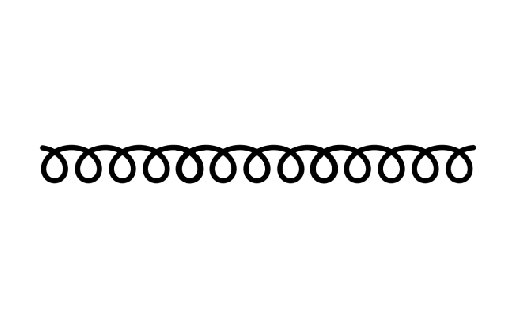
\includegraphics[scale=0.16, valign=c]{figs/diagrams/qcd_action/gluon_propagator})^{-1} +
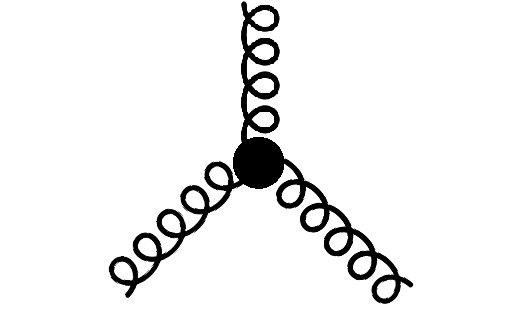
\includegraphics[scale=0.16, valign=c]{figs/diagrams/qcd_action/3gluon_vertex} +
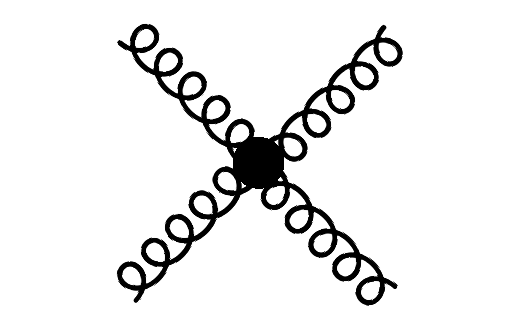
\includegraphics[scale=0.16, valign=c]{figs/diagrams/qcd_action/4gluon_vertex} +
(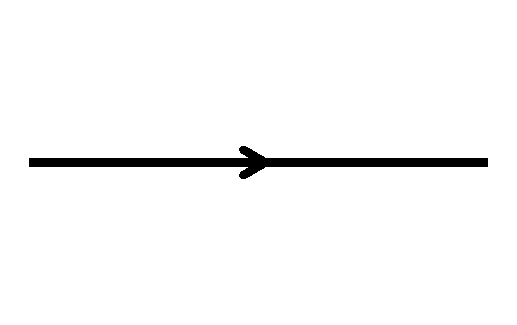
\includegraphics[scale=0.16, valign=c]{figs/diagrams/qcd_action/quark_propagator})^{-1} +
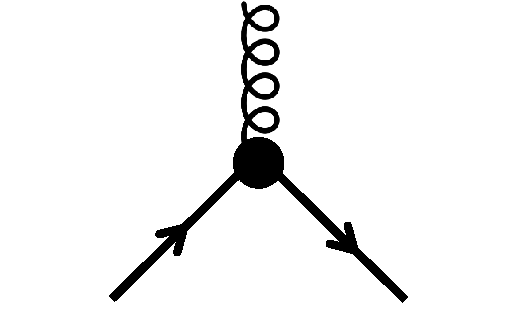
\includegraphics[scale=0.16, valign=c]{figs/diagrams/qcd_action/quark_gluon_vertex} +
(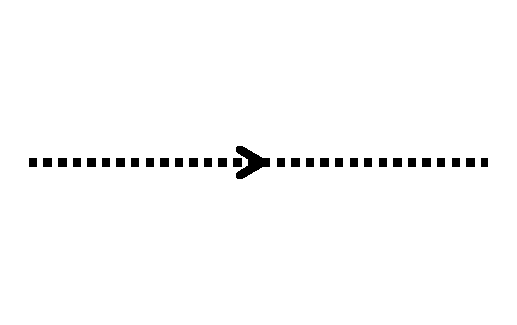
\includegraphics[scale=0.16, valign=c]{figs/diagrams/qcd_action/ghost_propagator})^{-1} +
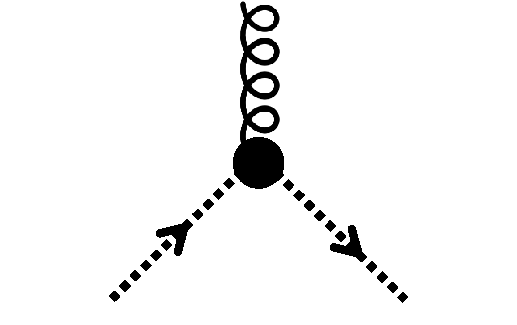
\includegraphics[scale=0.16, valign=c]{figs/diagrams/qcd_action/ghost_gluon_vertex}
\end{align*}

\caption{Diagrammatical representation of the QCD action. Compared to the Yang-Mills case we find in addition the (inverse) quark and ghost propagators and the respective interaction vertices with the gluons.}
\label{fig:S_QCD}
\end{figure}

\section{Dyson-Schwinger Equations for Yang-Mills and QCD}\label{sec:ym_qcd_dse}
Combining the results introduced in the two previous chapters, we now want to finally discuss, at least schematically, the functional relations that will be of great importance for the remainder of this work.\\
The quark propagator DSE\footnote{The addition \enquote{propagator} will be left out occasionally throughout this thesis, using \enquote{quark (gluon/ghost) DSE} synonymously to \enquote{quark (gluon/ghost) propagator DSE} if not explicitly stated otherwise.} can be derived from the master DSE (\ref{eqn:DSE}), this time using the QCD action (\ref{eqn:S_QCD}), the same way as explained for the scalar case earlier. Schematically it reads
\begin{equation}
\Gamma_{q \bar{q}}^{(2)}=S_{q \bar{q}}^{(2)}-S_{q \bar{q} A}^{(3)} \cdot G_{q} \cdot \Gamma_{q \bar{q} A}^{(3)} \cdot G_{A},\label{eqn:quark_DSE}
\end{equation}
with the quark and gluon propagators $G_q$ and $G_A$, and the classical and full quark-gluon vertices $S_{q \bar{q} A}^{(3)}$ and $\Gamma_{q \bar{q} A}^{(3)}$. As before, a diagrammatical representation of this equation is presented in \figref{fig:quarkDSE} at the beginning of the next page. It relates the full (inverse) two-point function to the bare propagator plus higher loop order diagrams, in our case the one-loop quark self energy $\Sigma_q$.\\
 We will postpone the discussion about regularization and renormalization of the diagrams to the main part of this work, where we will guide the reader step by step through the entire process of accessing the spectral functions from the DSE. \\
 The attentive reader might notice, that the quark DSE also needs the gluon propagator and the quark-gluon vertex as non-trivial external input. For the gluon propagator $G_A$, there has been a lot of progress in recent years, mainly with the help of reconstruction techniques, cf. \cite{Cyrol2017, CyrolMitterPawlowskiStrodthoff2017, CyrolPawlowskiRothkopWink2018}, and also just recently via the spectral approach used in this work. Note that the results we are stating here are partially not yet published. Details of the chosen external input will again be discussed in the respective chapter. 
The full vertex could in principle also be included via its spectral representation in this setting, but for a first attempt, it is approximated as the classical quark-gluon vertex, i.\,e. $\Gamma^{(3)} = S^{(3)}$.\\
To conclude our discussion, we will present the respective equations for the Yang-Mills sector in the following. The gluon DSE schematically reads
\begin{equation}
\Gamma_{A A}^{(2)}=S_{A A}^{(2)}-\frac{1}{2} S_{A A A}^{(3)} \cdot G_{A} \cdot \Gamma_{A A A}^{(3)} \cdot G_{A}+ \frac{1}{2}S_{c \bar{c} A}^{(3)} \cdot G_{c} \cdot \Gamma_{c \bar{c} A}^{(3)} \cdot G_{c}+ \text{higher loops}.\label{eqn:gluon_DSE}
\end{equation}
It inherits the same problem as the quark DSE, since it depends on the external input of the ghost propagator and the respective vertex, and vice versa for the ghost DSE. Therefore we have to deal with a dynamically coupled system of equations. This is already the main difference to the scalar case discussed in \chapref{chap:methods}, i.\,e. the appearance of a second field complicates the structure of the equations already a lot. Note also, that for the gluon DSE we only presented the expression up to one loop for feasibility. Solving this system for the Yang-Mills case only was the purpose of the work put forward in \cite{Horak2019}.\\ 
Although it is not directly important for our explicit calculations, for the sake of completeness, we also give the expression for the ghost propagator DSE,
\begin{equation}
\Gamma_{c \bar{c}}^{(2)}=S_{c \bar{c}}^{(2)}-S_{c \bar{c} A}^{(3)} \cdot G_{c} \cdot \Gamma_{c \bar{c} A}^{(3)} \cdot G_{A},\label{eqn:ghost_DSE}
\end{equation}
which looks very similar to the quark DSE. Here, the only non-trivial contribution is given by the ghost self-energy $\Sigma_c$. In an analogous analysis of the ghost DSE as compared to our work, spectral functions could be successfully computed. The results have just been published recently by group members and collaborators, cf. \cite{HorakPapavassiliouPawlowskiWink2021}. In analogy to the quark DSE, we present the respective diagrammatical representations of the gluon and ghost DSEs in \figref{fig:YM_DSEs}.\\

\begin{figure}[t]
\centering
\begin{align*}
\bigg(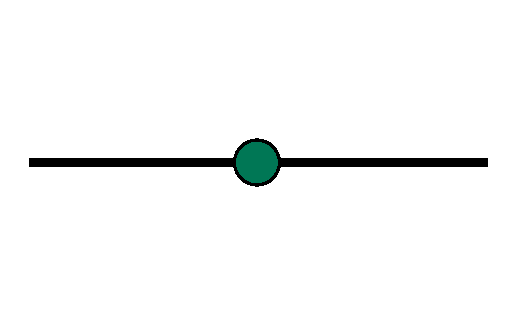
\includegraphics[scale=0.4, valign=c]{figs/diagrams/quarkDSE/full_quark_propagator}\bigg)^{-1} = 
\bigg(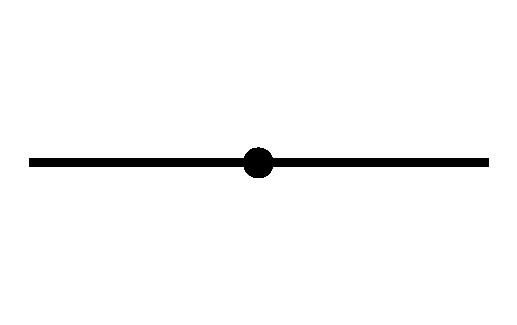
\includegraphics[scale=0.4, valign=c]{figs/diagrams/quarkDSE/bare_quark_propagator.pdf}\bigg)^{-1} - 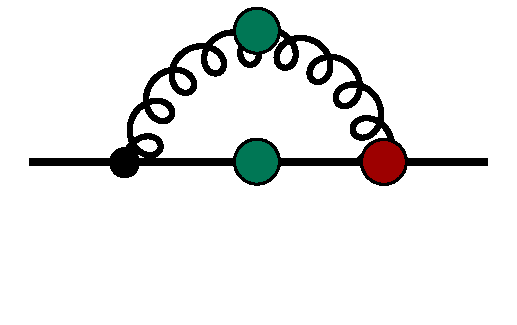
\includegraphics[scale=0.4, valign=c]{figs/diagrams/quarkDSE/quark_self_energy}
\end{align*}

\caption{Diagrammatic representation of the quark propagator DSE, often referred to as the quark gap equation. The non-trivial contribution is given by the one-loop quark self energy $\Sigma_q$.}
\label{fig:quarkDSE}
\end{figure}
\newpage
\begin{figure}[H]
\centering
\begin{align*}
\bigg(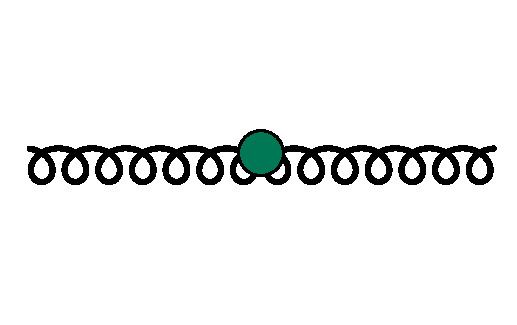
\includegraphics[scale=0.3, valign=c]{figs/diagrams/gluonDSE/full_gluon_propagator}\bigg)^{-1} &= 
\bigg(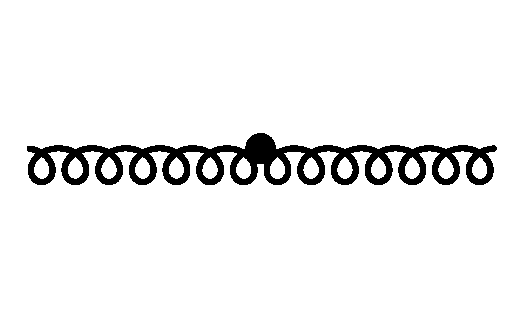
\includegraphics[scale=0.3, valign=c]{figs/diagrams/gluonDSE/bare_gluon_propagator.pdf}\bigg)^{-1}\ - \frac{1}{2}\ 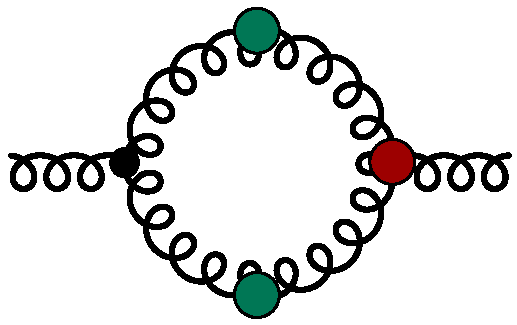
\includegraphics[scale=0.3, valign=c]{figs/diagrams/gluonDSE/gluon_polarization}\ +\ \frac{1}{2}\ 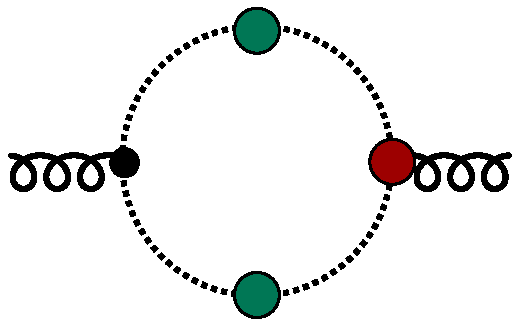
\includegraphics[scale=0.3, valign=c]{figs/diagrams/gluonDSE/ghost_polarization}  \\[0.8em]
\bigg(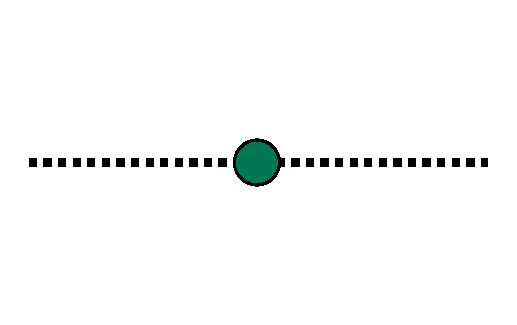
\includegraphics[scale=0.3, valign=c]{figs/diagrams/ghostDSE/full_ghost_propagator}\bigg)^{-1} &= 
\bigg(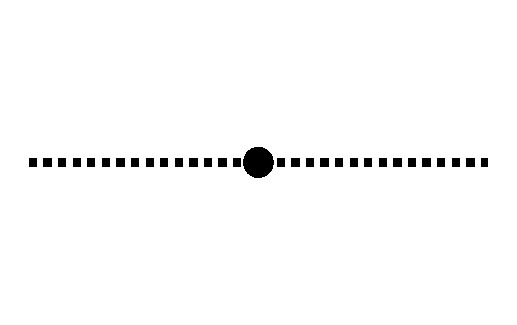
\includegraphics[scale=0.3, valign=c]{figs/diagrams/ghostDSE/bare_ghost_propagator.pdf}\bigg)^{-1}\hspace{0.625em} -\hspace{0.625em}   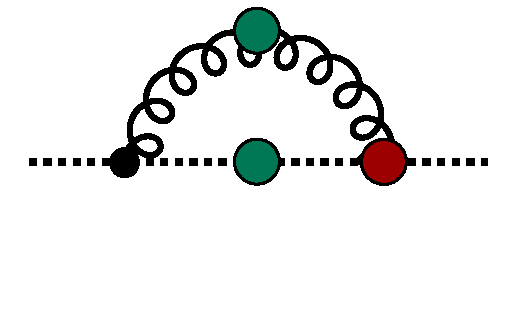
\includegraphics[scale=0.3, valign=c]{figs/diagrams/ghostDSE/ghost_self_energy} \\[0.8em]
\bigg(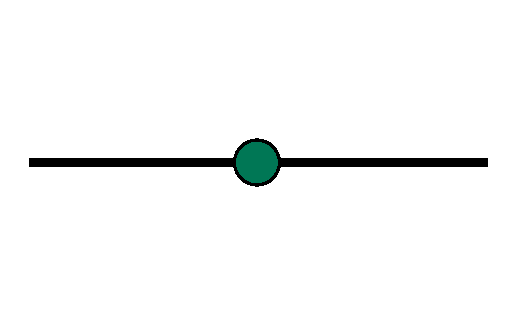
\includegraphics[scale=0.3, valign=c]{figs/diagrams/quarkDSE/full_quark_propagator}\bigg)^{-1} &= 
\bigg(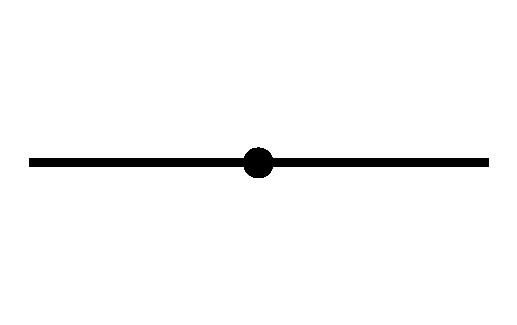
\includegraphics[scale=0.3, valign=c]{figs/diagrams/quarkDSE/bare_quark_propagator.pdf}\bigg)^{-1}\hspace{0.625em} -\hspace{0.625em} 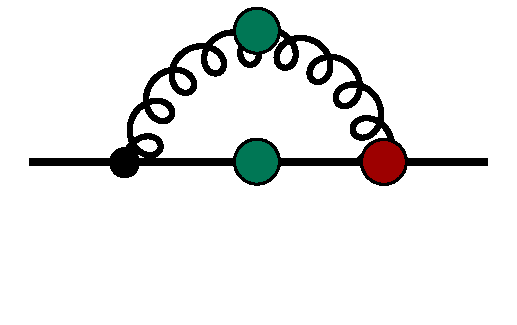
\includegraphics[scale=0.3, valign=c]{figs/diagrams/quarkDSE/quark_self_energy}
\end{align*}

\caption{Diagrammatical representation of the gluon and ghost propagator DSEs according to equations (\ref{eqn:gluon_DSE}) and (\ref{eqn:ghost_DSE}). The gluon DSE is truncated at one loop.}
\label{fig:YM_DSEs}
\end{figure}

